% Options for packages loaded elsewhere
\PassOptionsToPackage{unicode}{hyperref}
\PassOptionsToPackage{hyphens}{url}
%
\documentclass[
  12pt,
]{article}
\usepackage{amsmath,amssymb}
\usepackage{lmodern}
\usepackage{ifxetex,ifluatex}
\ifnum 0\ifxetex 1\fi\ifluatex 1\fi=0 % if pdftex
  \usepackage[T1]{fontenc}
  \usepackage[utf8]{inputenc}
  \usepackage{textcomp} % provide euro and other symbols
\else % if luatex or xetex
  \usepackage{unicode-math}
  \defaultfontfeatures{Scale=MatchLowercase}
  \defaultfontfeatures[\rmfamily]{Ligatures=TeX,Scale=1}
\fi
% Use upquote if available, for straight quotes in verbatim environments
\IfFileExists{upquote.sty}{\usepackage{upquote}}{}
\IfFileExists{microtype.sty}{% use microtype if available
  \usepackage[]{microtype}
  \UseMicrotypeSet[protrusion]{basicmath} % disable protrusion for tt fonts
}{}
\makeatletter
\@ifundefined{KOMAClassName}{% if non-KOMA class
  \IfFileExists{parskip.sty}{%
    \usepackage{parskip}
  }{% else
    \setlength{\parindent}{0pt}
    \setlength{\parskip}{6pt plus 2pt minus 1pt}}
}{% if KOMA class
  \KOMAoptions{parskip=half}}
\makeatother
\usepackage{xcolor}
\IfFileExists{xurl.sty}{\usepackage{xurl}}{} % add URL line breaks if available
\IfFileExists{bookmark.sty}{\usepackage{bookmark}}{\usepackage{hyperref}}
\hypersetup{
  pdftitle={Homework 1 - Truth Tables \& Linear Programming with AMPL},
  pdfauthor={Daniel Carpenter and Effouehi Moody},
  hidelinks,
  pdfcreator={LaTeX via pandoc}}
\urlstyle{same} % disable monospaced font for URLs
\usepackage[margin=1in]{geometry}
\usepackage{graphicx}
\makeatletter
\def\maxwidth{\ifdim\Gin@nat@width>\linewidth\linewidth\else\Gin@nat@width\fi}
\def\maxheight{\ifdim\Gin@nat@height>\textheight\textheight\else\Gin@nat@height\fi}
\makeatother
% Scale images if necessary, so that they will not overflow the page
% margins by default, and it is still possible to overwrite the defaults
% using explicit options in \includegraphics[width, height, ...]{}
\setkeys{Gin}{width=\maxwidth,height=\maxheight,keepaspectratio}
% Set default figure placement to htbp
\makeatletter
\def\fps@figure{htbp}
\makeatother
\setlength{\emergencystretch}{3em} % prevent overfull lines
\providecommand{\tightlist}{%
  \setlength{\itemsep}{0pt}\setlength{\parskip}{0pt}}
\setcounter{secnumdepth}{5}
\ifluatex
  \usepackage{selnolig}  % disable illegal ligatures
\fi

\title{Homework 1 - Truth Tables \& Linear Programming with AMPL}
\author{Daniel Carpenter and Effouehi Moody}
\date{January 2022}

\begin{document}
\maketitle

{
\setcounter{tocdepth}{2}
\tableofcontents
}
\begin{center}\rule{0.5\linewidth}{0.5pt}\end{center}

\hypertarget{problem-1}{%
\section{\texorpdfstring{Problem
\texttt{1}}{Problem 1}}\label{problem-1}}

\begin{center}\rule{0.5\linewidth}{0.5pt}\end{center}

\begin{figure}
\centering
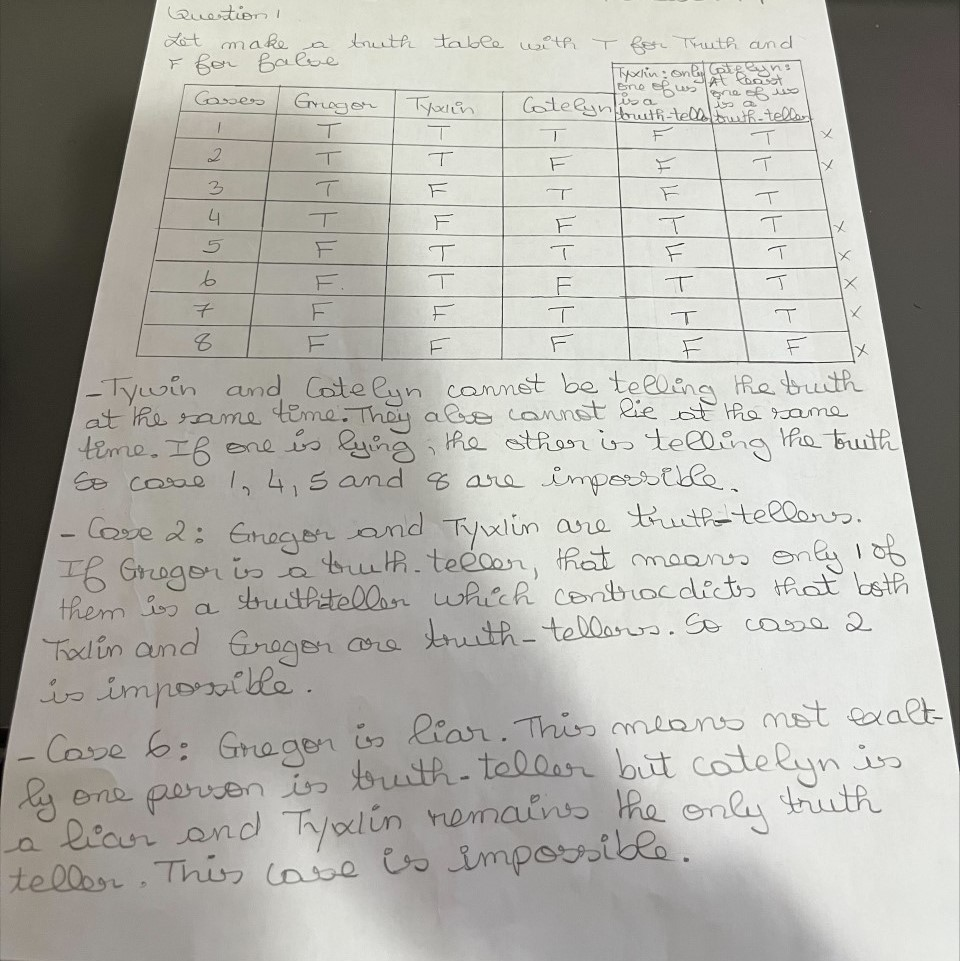
\includegraphics{"Output_Images/problem1.1.jpg}
\caption{Image}
\end{figure}

\begin{figure}
\centering
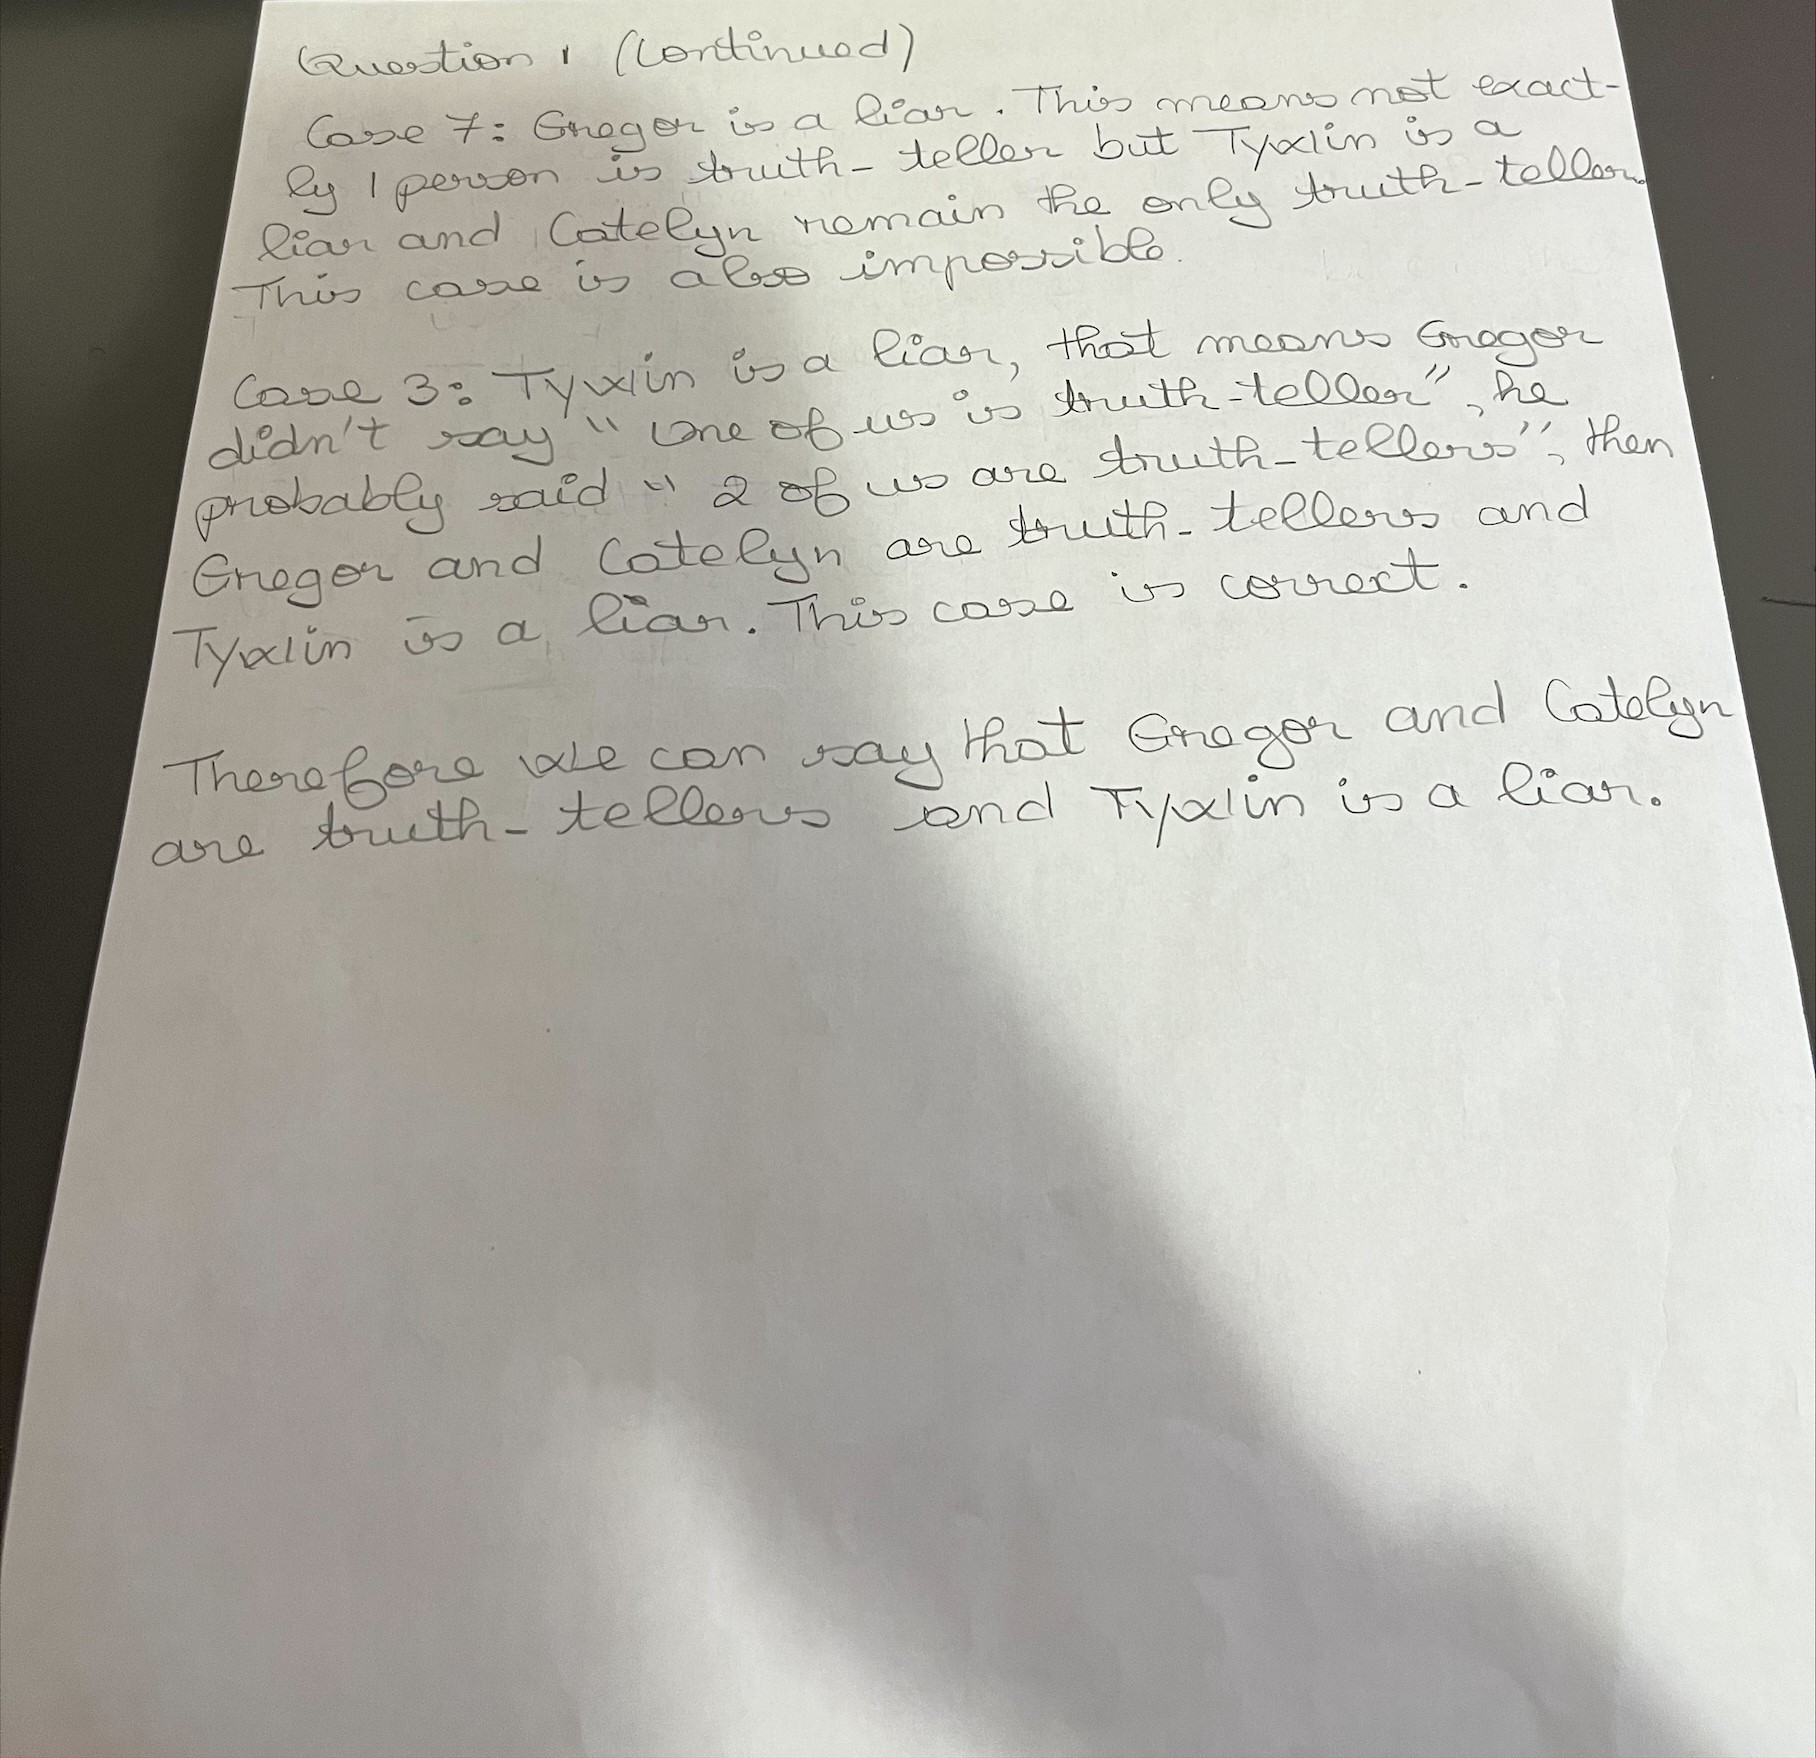
\includegraphics{"Output_Images/problem1.2.jpeg}
\caption{Image}
\end{figure}

\begin{center}\rule{0.5\linewidth}{0.5pt}\end{center}

\hypertarget{problem-2}{%
\section{\texorpdfstring{Problem
\texttt{2}}{Problem 2}}\label{problem-2}}

\begin{center}\rule{0.5\linewidth}{0.5pt}\end{center}

\begin{figure}
\centering
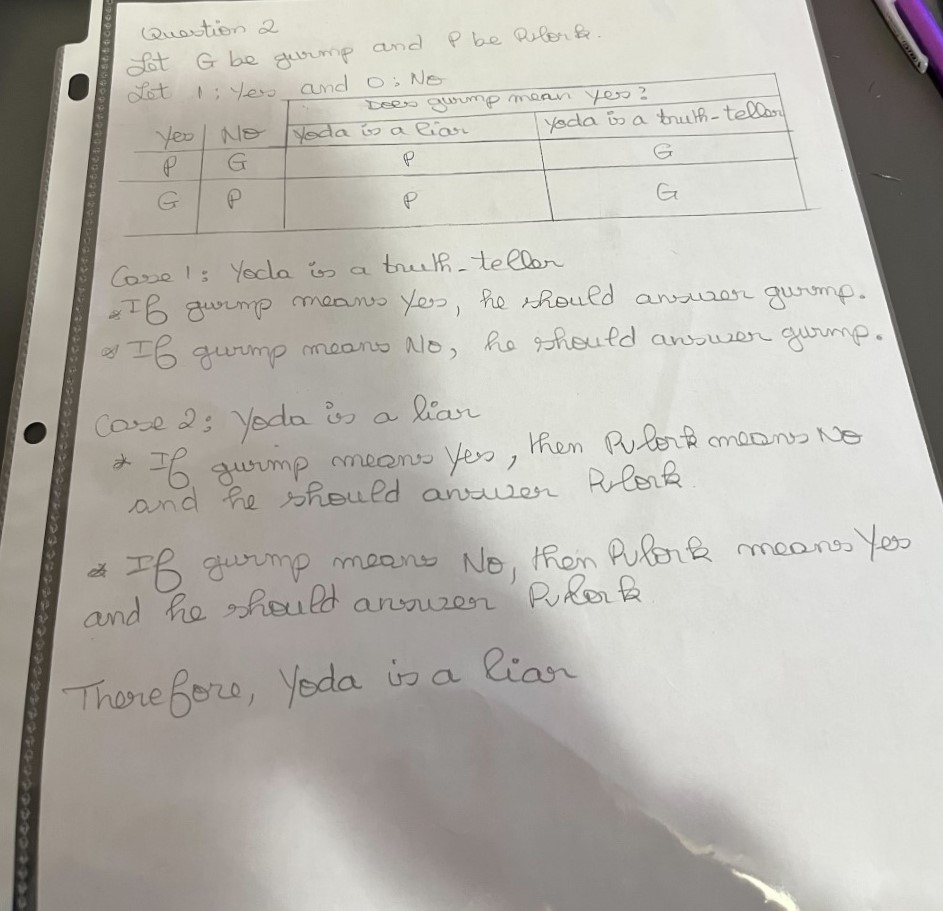
\includegraphics{"Output_Images/problem2.jpg}
\caption{Image}
\end{figure}

\hypertarget{problem-3}{%
\section{\texorpdfstring{Problem
\texttt{3}}{Problem 3}}\label{problem-3}}

\begin{center}\rule{0.5\linewidth}{0.5pt}\end{center}

\hypertarget{task-a}{%
\subsection{\texorpdfstring{Task \texttt{a}}{Task a}}\label{task-a}}

\hypertarget{decision-variables}{%
\subsubsection{Decision Variables}\label{decision-variables}}

\texttt{bondA}: dollars \(\in \mathbb{R}\) to invest in bond A\\
\texttt{bondB}: dollars \(\in \mathbb{R}\) to invest in bond B\\
\texttt{bondC}: dollars \(\in \mathbb{R}\) to invest in bond C\\
\texttt{bondD}: dollars \(\in \mathbb{R}\) to invest in bond D\\
\texttt{bondE}: dollars \(\in \mathbb{R}\) to invest in bond E

\hypertarget{objective-function}{%
\subsubsection{Objective Function}\label{objective-function}}

\begin{itemize}
\tightlist
\item
  Maximize the Expected Earnings of the portfolio
\end{itemize}

\[
Maximize \ Z = (0.043 \times bondA) + (0.027 \times bondB) + (0.025 \times bondC) + (0.022 \times bondD) + (0.045 \times bondE)
\]

\hypertarget{constraints}{%
\subsubsection{Constraints}\label{constraints}}

\textbf{C1:} Budget to invest is \$10 MM or less \[
budget: bondA + bondB + bondC + bondD + bondE \leq 10
\]

\textbf{C2:} At least \$4 million must be invested in government and
agency bonds \[
govtAndAgency: bondB + bondC + bondD \geq 4
\]

\textbf{C3:} Average Quality of the Portfolio must not exceed 1.4 \[
avgQuality: (0.6 \times bondA) + (0.6 \times bondB) - (0.4 \times bondC) 
- (0.4 \times bondD) + (3.6 \times bondE) \leq 0
\]

\textbf{C4:} The Average Maturity must not Exceed Five Years \[
avgMaturity: (4 \times bondA) + (10 \times bondB) - (1 \times bondC) 
- (2 \times bondD) - (3 \times bondE) \leq 0
\]

\hypertarget{code}{%
\subsubsection{Code}\label{code}}

\begin{figure}
\centering
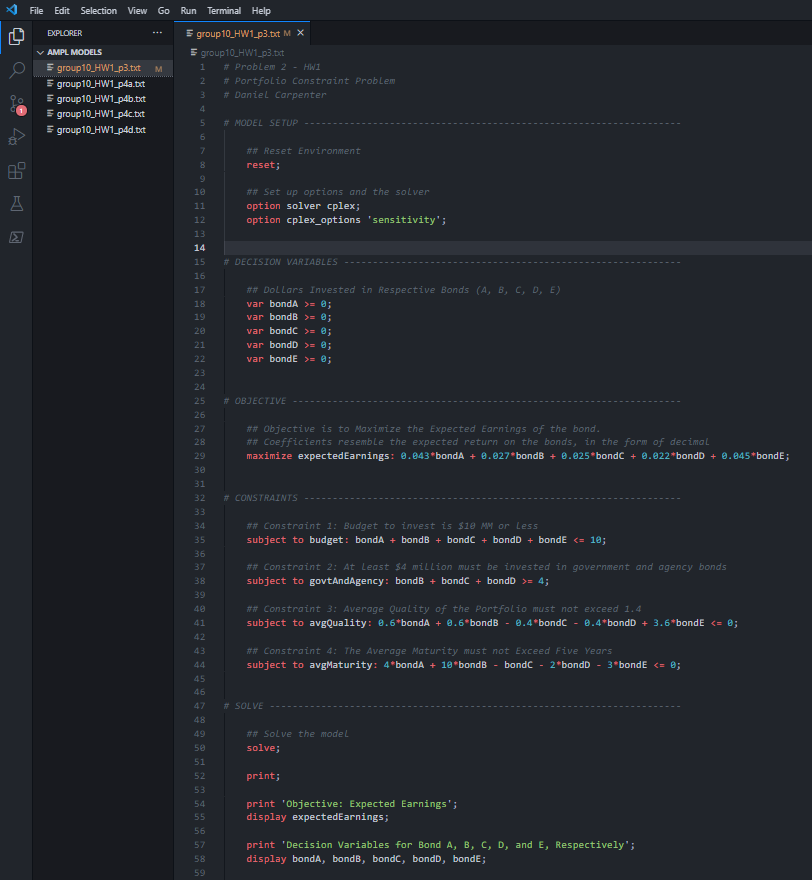
\includegraphics{"Output_Images/codeProblem3.png}
\caption{Image}
\end{figure}

\hypertarget{output}{%
\subsubsection{Output}\label{output}}

\begin{figure}
\centering
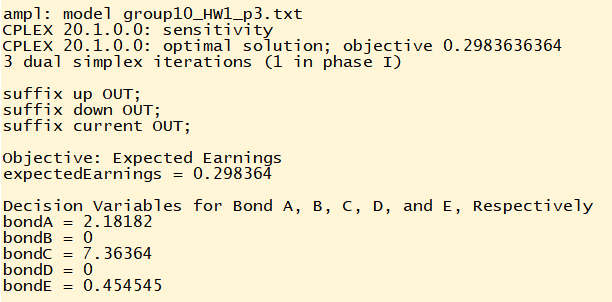
\includegraphics{"Output_Images/outputProblem3.png}
\caption{Image}
\end{figure}

\begin{center}\rule{0.5\linewidth}{0.5pt}\end{center}

\hypertarget{problem-4}{%
\section{\texorpdfstring{Problem
\texttt{4}}{Problem 4}}\label{problem-4}}

\begin{center}\rule{0.5\linewidth}{0.5pt}\end{center}

\hypertarget{task-a-1}{%
\subsection{\texorpdfstring{Task \texttt{a}}{Task a}}\label{task-a-1}}

\hypertarget{decision-variables-1}{%
\subsubsection{Decision Variables}\label{decision-variables-1}}

\texttt{tv} = the number of minutes \(\in \mathbb{R}\) to air
advertising on the \emph{television} medium\\
\texttt{magazine} = the number of pages \(\in \mathbb{I}\) to to
advertise on the \emph{magazine} medium

\hypertarget{objective-function-1}{%
\subsubsection{Objective Function}\label{objective-function-1}}

\begin{itemize}
\tightlist
\item
  Maximize the total audience reach
\end{itemize}

\[
Maximize \ Z = (1.8\times tv) + (1.0 \times magazine)
\]

\hypertarget{constraints-1}{%
\subsubsection{Constraints}\label{constraints-1}}

\textbf{C1}: Must not Exceed Budget of 1 Million dollars\\
\[
budget: (20,000 \times tv) + (10,000 \times magazine) \leq 1,000,000
\]

\textbf{C2}: Must have at least 10 minutes of air time on the TV
medium\\
\[
minTimeTV: tv \geq 10
\]

\hypertarget{code-1}{%
\subsubsection{Code}\label{code-1}}

\begin{figure}
\centering
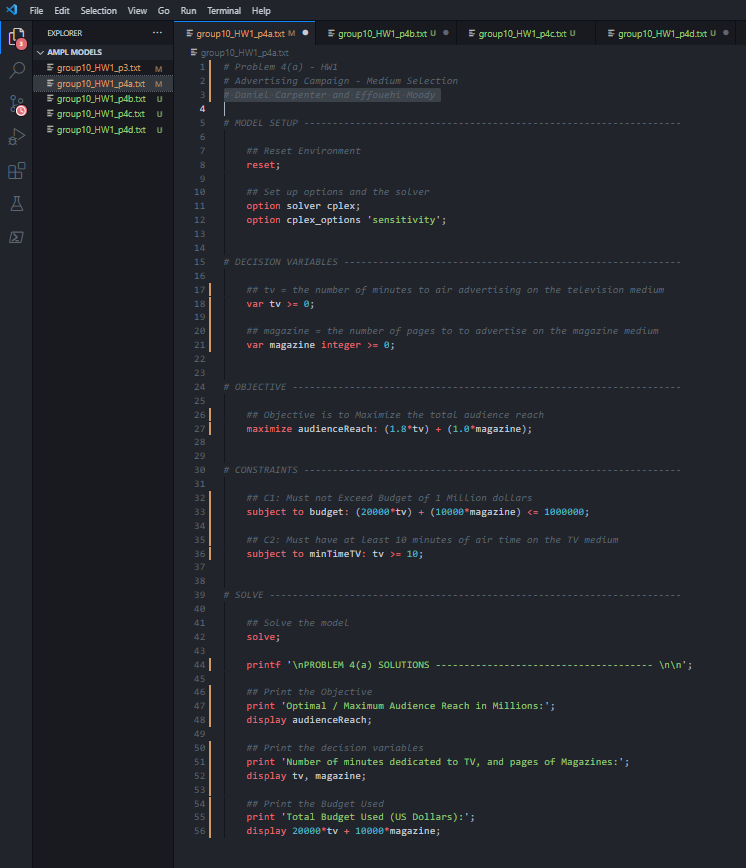
\includegraphics{"Output_Images/codeProblem4a.png}
\caption{Image}
\end{figure}

\hypertarget{output-1}{%
\subsubsection{Output}\label{output-1}}

\begin{figure}
\centering
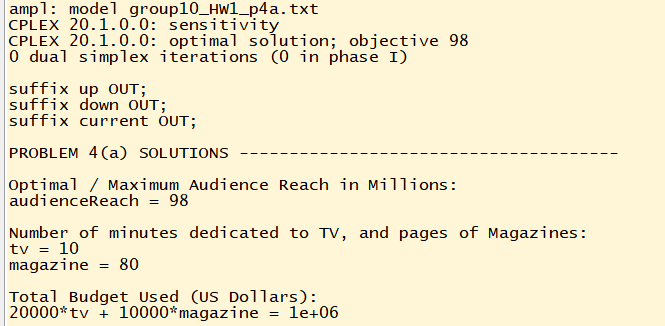
\includegraphics{"Output_Images/group10_HW1_p4a.txt OUTPUT.png}
\caption{Image}
\end{figure}

\hypertarget{solving-problem-4a-graphically-by-hand}{%
\subsubsection{\texorpdfstring{Solving Problem \texttt{4(a)} Graphically
by
Hand}{Solving Problem 4(a) Graphically by Hand}}\label{solving-problem-4a-graphically-by-hand}}

\begin{figure}
\centering
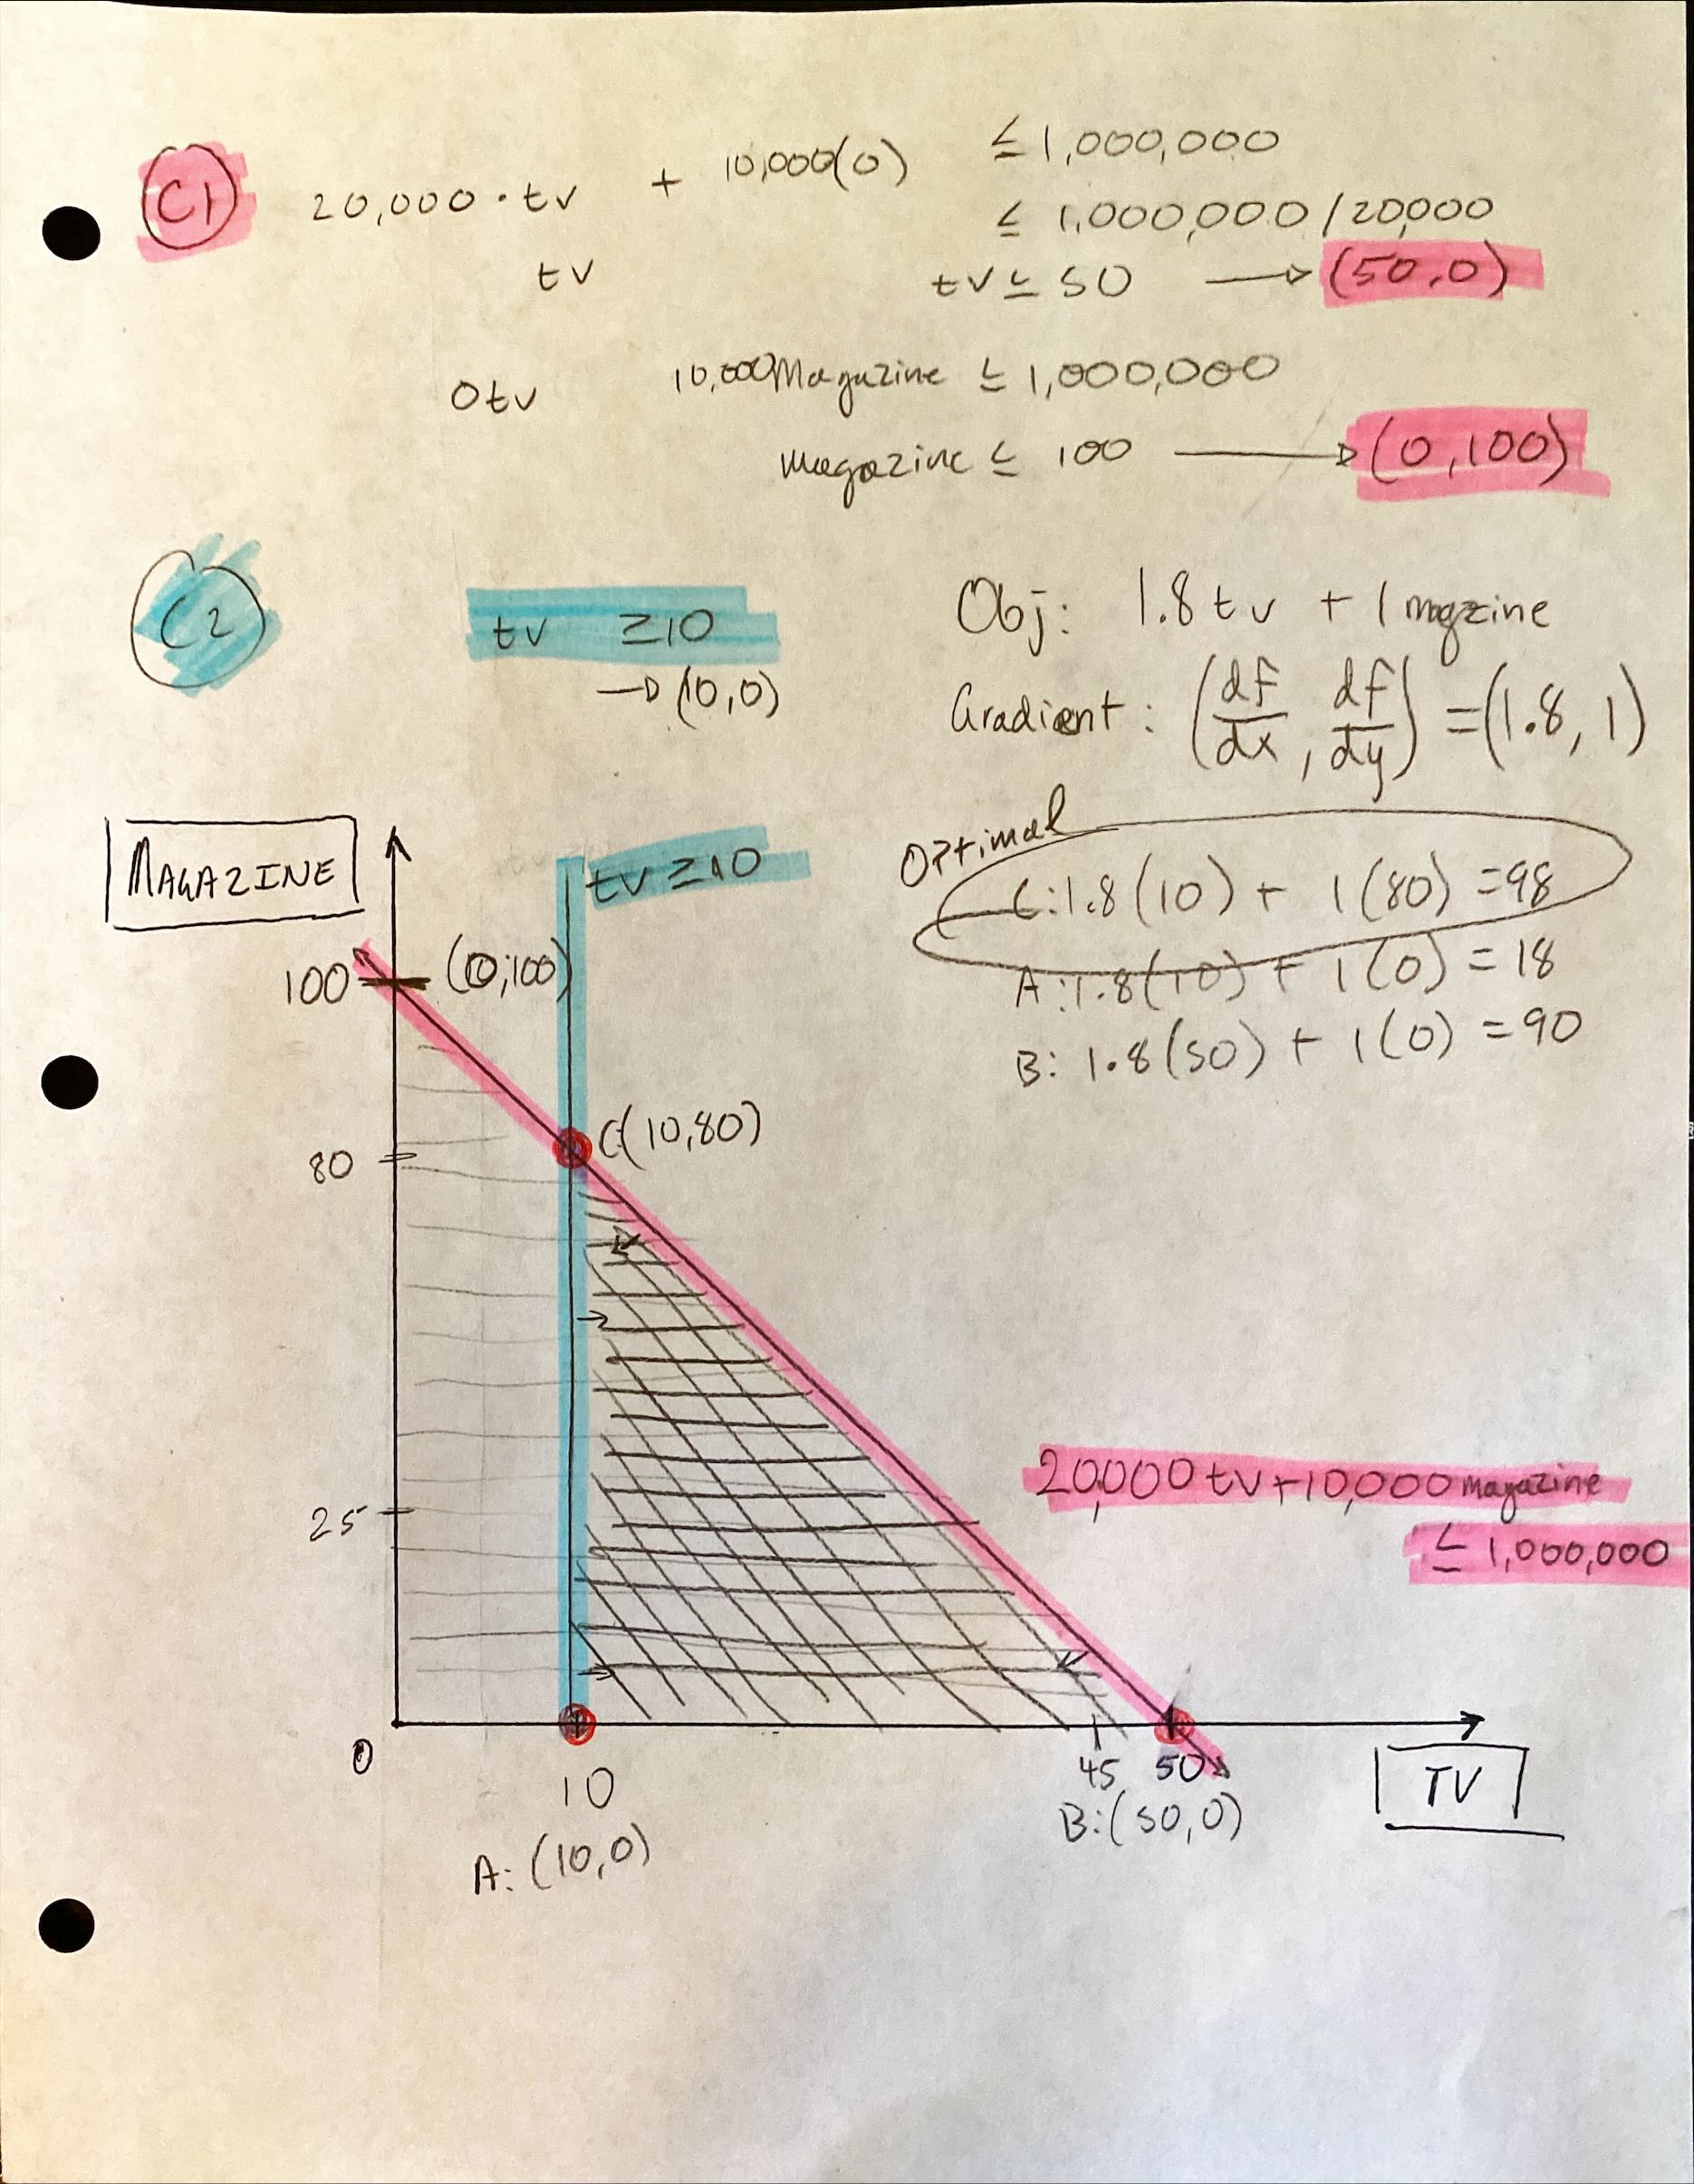
\includegraphics{"Output_Images/problem4a.1.jpg}
\caption{Image}
\end{figure}

\begin{center}\rule{0.5\linewidth}{0.5pt}\end{center}

\hypertarget{task-b}{%
\subsection{\texorpdfstring{Task \texttt{b}}{Task b}}\label{task-b}}

\hypertarget{additional-constraint-labor-time}{%
\subsubsection{Additional Constraint: Labor
Time}\label{additional-constraint-labor-time}}

\textbf{C3}: Only 100 person weeks available, given it takes three weeks
and one week to create a \texttt{tv} and \texttt{magazine} minute for
advertisement, respectively.\\
\[
personWeeks: (3 \times tv) + (1 \times magazine) \leq 100
\]

\hypertarget{code-2}{%
\subsubsection{Code}\label{code-2}}

\begin{figure}
\centering
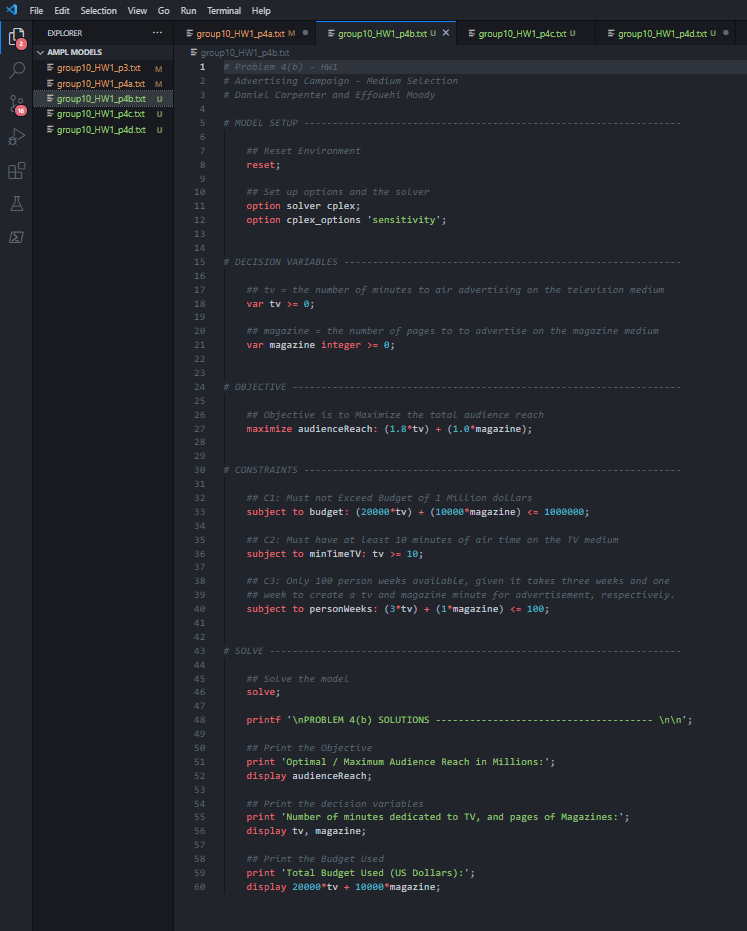
\includegraphics{"Output_Images/codeProblem4b.png}
\caption{Image}
\end{figure}

\hypertarget{output-2}{%
\subsubsection{Output}\label{output-2}}

\begin{figure}
\centering
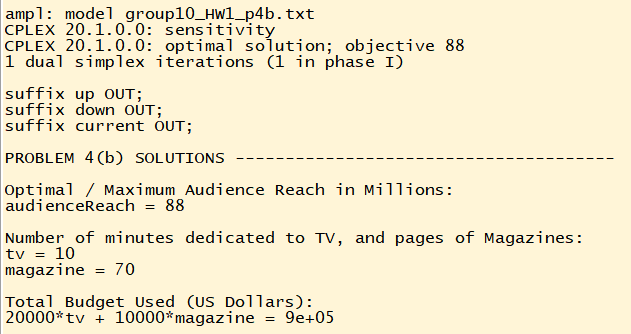
\includegraphics{"Output_Images/group10_HW1_p4b.txt OUTPUT.png}
\caption{Image}
\end{figure}

\begin{center}\rule{0.5\linewidth}{0.5pt}\end{center}

\hypertarget{task-c}{%
\subsection{\texorpdfstring{Task \texttt{c}}{Task c}}\label{task-c}}

\hypertarget{additional-constraint-radio-advertising-medium}{%
\subsubsection{Additional Constraint: Radio Advertising
Medium}\label{additional-constraint-radio-advertising-medium}}

\hypertarget{decision-variables-2}{%
\subsubsection{Decision Variables}\label{decision-variables-2}}

\texttt{tv} = the number of minutes \(\in \mathbb{R}\) to air
advertising on the \emph{television} medium\\
\texttt{magazine} = the number of pages \(\in \mathbb{I}\) to to
advertise on the \emph{magazine} medium \texttt{radio} = the number of
minutes \(\in \mathbb{R}\) to air advertising on the \emph{radio} medium

\hypertarget{objective-function-2}{%
\subsubsection{Objective Function}\label{objective-function-2}}

\begin{itemize}
\tightlist
\item
  Maximize the total audience reach
\end{itemize}

\[
Maximize \ Z = (1.80\times tv) + (1.00 \times magazine) + (0.25 \times radio)
\]

\hypertarget{new-constraints}{%
\subsubsection{New Constraints}\label{new-constraints}}

\textbf{C1}: Must not Exceed Budget of 1 Million dollars \[
budget: (20,000 \times tv) + (10,000 \times magazine) + (2,000 \times radio) \leq 1,000,000
\]

\textbf{C2}: Must have at least 10 minutes of air time on the TV
medium\\
\[
minTimeTV: tv \geq 10
\]

\textbf{C3}: Only 100 person weeks available, given it takes three weeks
and one week to create a \texttt{tv} and \texttt{magazine} minute for
advertisement, respectively. It only takes one day for \texttt{radio}.\\
\[
personWeeks: (3 \times tv) + (1 \times magazine) + (\frac{1}{7} \times radio) \leq 100
\]

\hypertarget{code-3}{%
\subsubsection{Code}\label{code-3}}

\begin{figure}
\centering
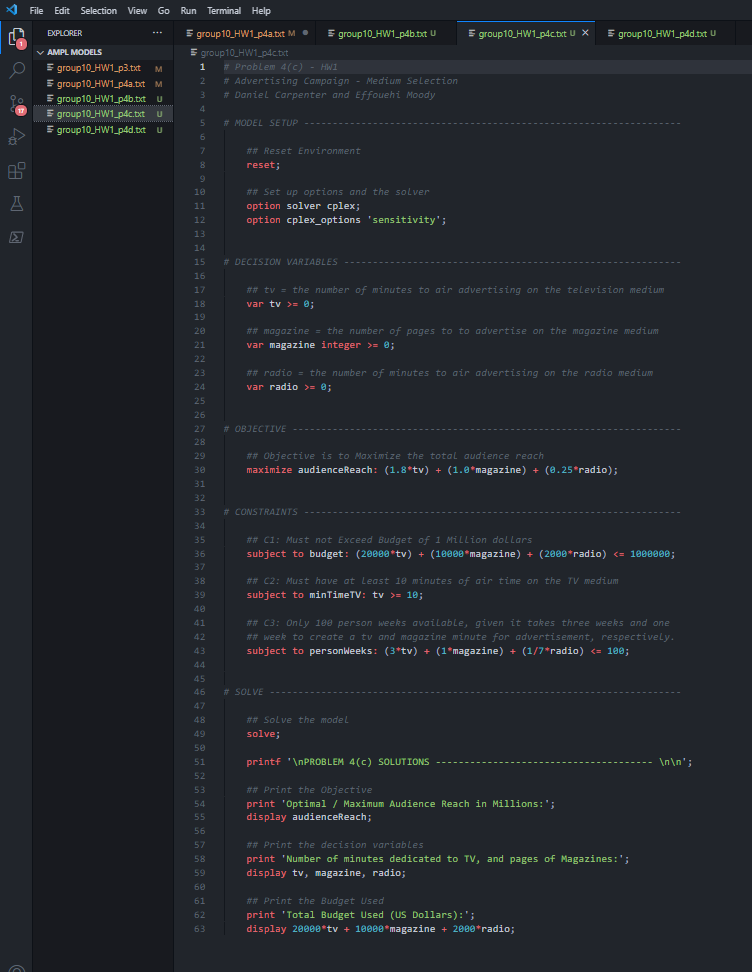
\includegraphics{"Output_Images/codeProblem4c.png}
\caption{Image}
\end{figure}

\hypertarget{output-3}{%
\subsubsection{Output}\label{output-3}}

\begin{figure}
\centering
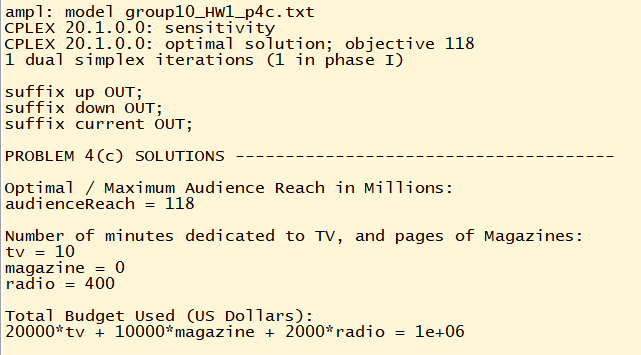
\includegraphics{"Output_Images/group10_HW1_p4c.txt OUTPUT.png}
\caption{Image}
\end{figure}

\begin{center}\rule{0.5\linewidth}{0.5pt}\end{center}

\hypertarget{task-d}{%
\subsection{\texorpdfstring{Task \texttt{d}}{Task d}}\label{task-d}}

\hypertarget{additional-constraints-miminum-magazine-and-maximum-radio-requirements}{%
\subsubsection{Additional Constraints: Miminum Magazine and Maximum
Radio
Requirements}\label{additional-constraints-miminum-magazine-and-maximum-radio-requirements}}

\textbf{C4}: Must sign up for at least 2 magazine pages \[
minMagazines: magazine \geq 2
\]

\textbf{C5}: Must to exceed 120 minutes of radio \[
maxRadio: radio \leq 120
\]

\hypertarget{code-4}{%
\subsubsection{Code}\label{code-4}}

\begin{figure}
\centering
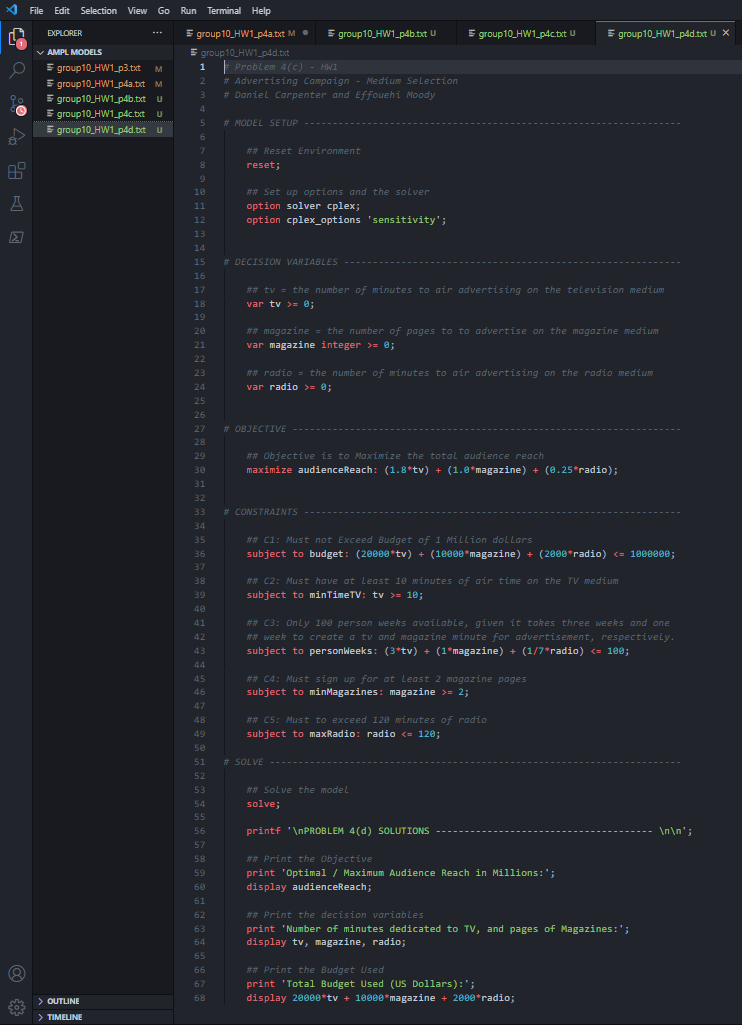
\includegraphics{"Output_Images/codeProblem4d.png}
\caption{Image}
\end{figure}

\hypertarget{output-4}{%
\subsubsection{Output}\label{output-4}}

\begin{figure}
\centering
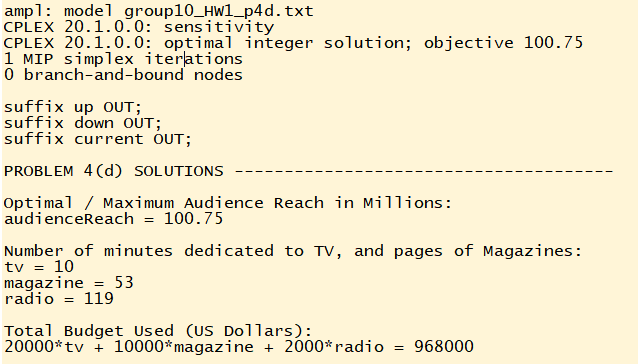
\includegraphics{"Output_Images/group10_HW1_p4d.txt OUTPUT.png}
\caption{Image}
\end{figure}

\begin{center}\rule{0.5\linewidth}{0.5pt}\end{center}

\hypertarget{problem-5}{%
\section{\texorpdfstring{Problem
\texttt{5}}{Problem 5}}\label{problem-5}}

\begin{center}\rule{0.5\linewidth}{0.5pt}\end{center}

\hypertarget{base-mathematical-formulation-and-code}{%
\subsection{Base Mathematical Formulation and
Code}\label{base-mathematical-formulation-and-code}}

\begin{itemize}
\tightlist
\item
  \emph{Each task shows a separate change to the base model. Therefore,
  each change should not accumulate.}
\end{itemize}

\hypertarget{mathematical-formulation}{%
\subsubsection{Mathematical
Formulation}\label{mathematical-formulation}}

\begin{figure}
\centering
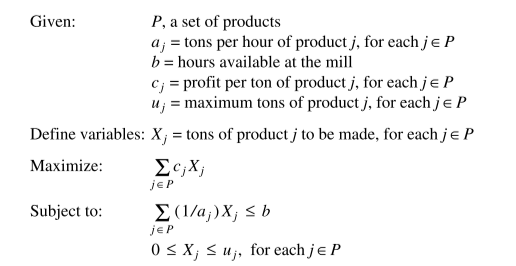
\includegraphics{"Output_Images/mathProblem5.png}
\caption{Image}
\end{figure}

\hypertarget{code-for-model-.mod-and-input-data-.dat}{%
\subsubsection{\texorpdfstring{Code for Model \texttt{.mod} and Input
Data
\texttt{.dat}}{Code for Model .mod and Input Data .dat}}\label{code-for-model-.mod-and-input-data-.dat}}

\begin{figure}
\centering
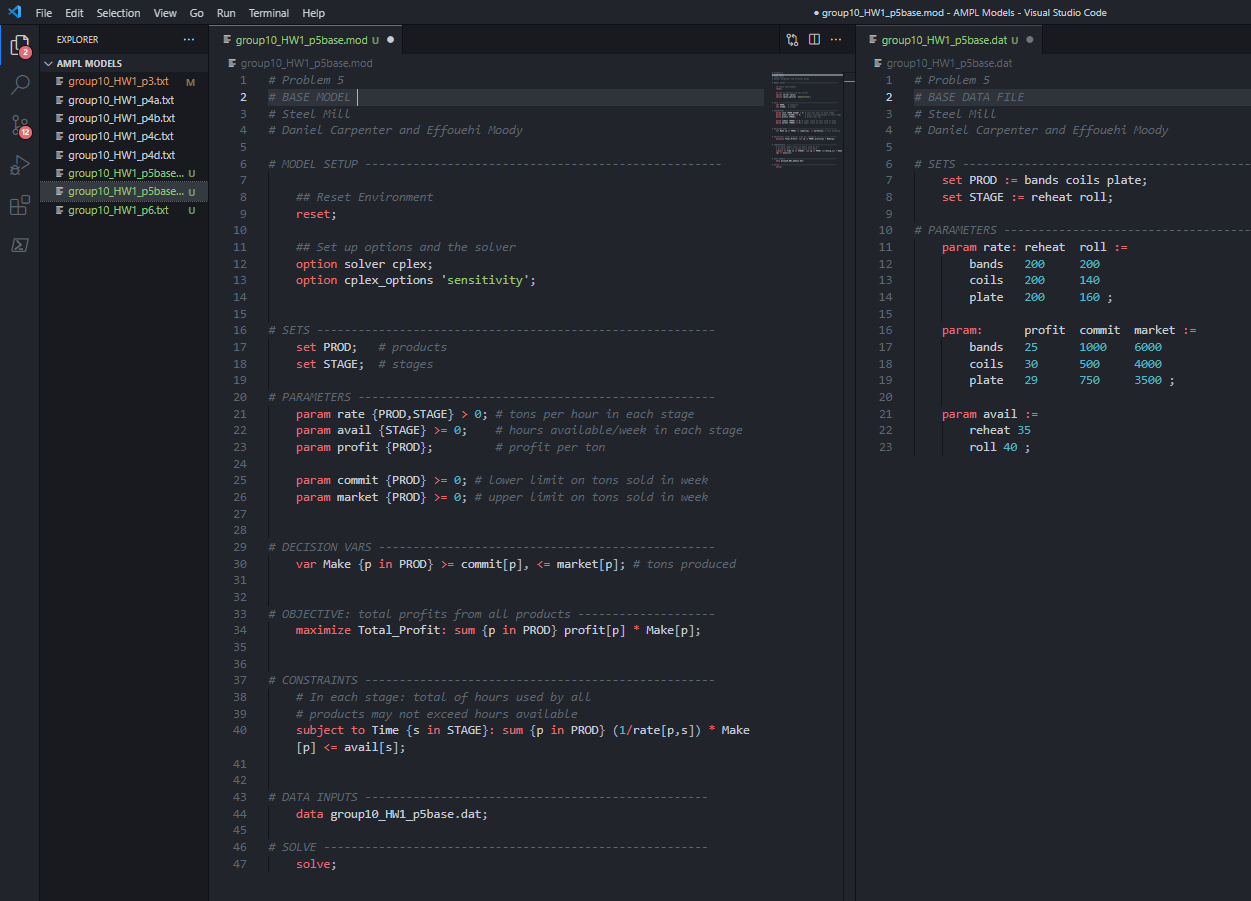
\includegraphics{"Output_Images/codeProblem5base.png}
\caption{Image}
\end{figure}

\hypertarget{task-a-2}{%
\subsection{\texorpdfstring{Task \texttt{a}}{Task a}}\label{task-a-2}}

\hypertarget{changed-constraint-for-total-hours}{%
\subsubsection{Changed Constraint for Total
Hours}\label{changed-constraint-for-total-hours}}

\begin{itemize}
\tightlist
\item
  \emph{Change the constraints so that total hours used by all products
  must equal the total hours available for each stage}
\end{itemize}

\hypertarget{code-5}{%
\subsubsection{Code}\label{code-5}}

\begin{figure}
\centering
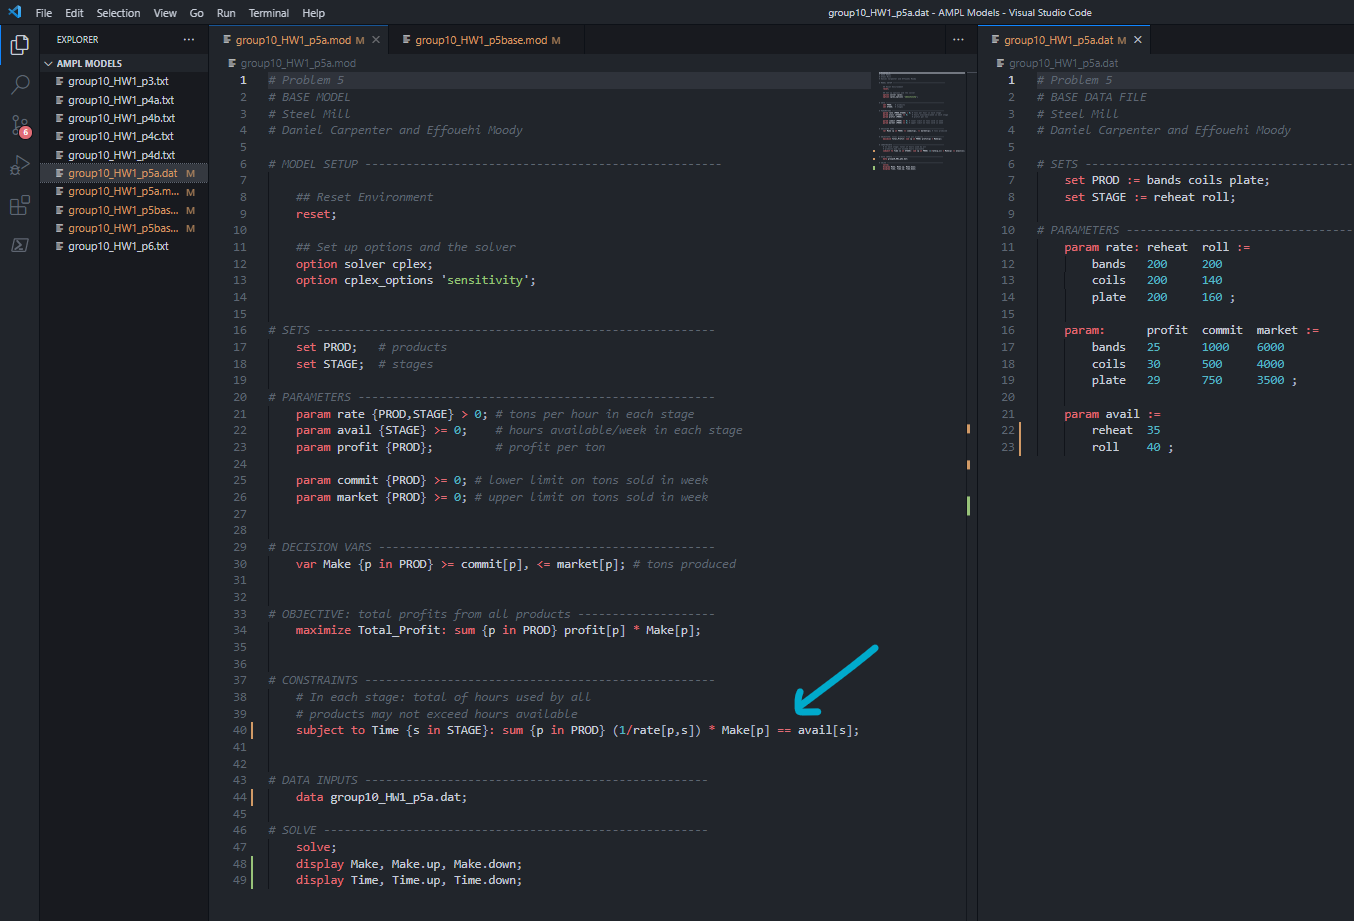
\includegraphics{"Output_Images/codeProblem5a.png}
\caption{Image}
\end{figure}

\hypertarget{output-5}{%
\subsubsection{Output}\label{output-5}}

\begin{quote}
There is no difference in the optimal solution because the range of Time
before there is a change in optimal remains the same, and the hours
available have not changed.
\end{quote}

\begin{figure}
\centering
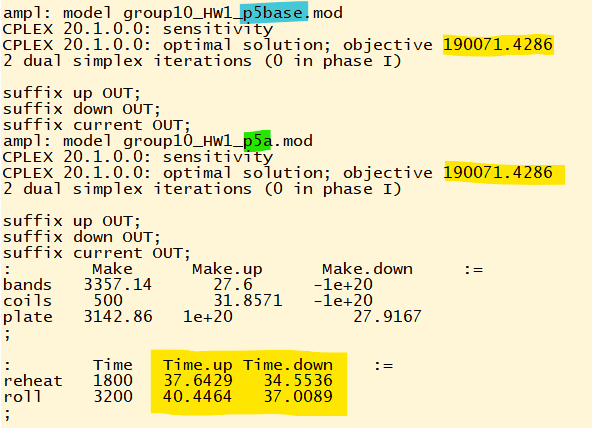
\includegraphics{"Output_Images/outputProblem5a.png}
\caption{Image}
\end{figure}

\hypertarget{task-b-1}{%
\subsection{\texorpdfstring{Task \texttt{b}}{Task b}}\label{task-b-1}}

\hypertarget{new-constraint-for-max-weight}{%
\subsubsection{New Constraint for Max
Weight}\label{new-constraint-for-max-weight}}

\begin{itemize}
\tightlist
\item
  \emph{Restrict the total weight of all products to be less than a new
  parameter, max\_weight = 6,500}
\end{itemize}

\[
totalWeight: \sum_{p \ \in \ PROD} Make_{p} \leq max\_weight
\]

\hypertarget{code-6}{%
\subsubsection{Code}\label{code-6}}

\begin{figure}
\centering
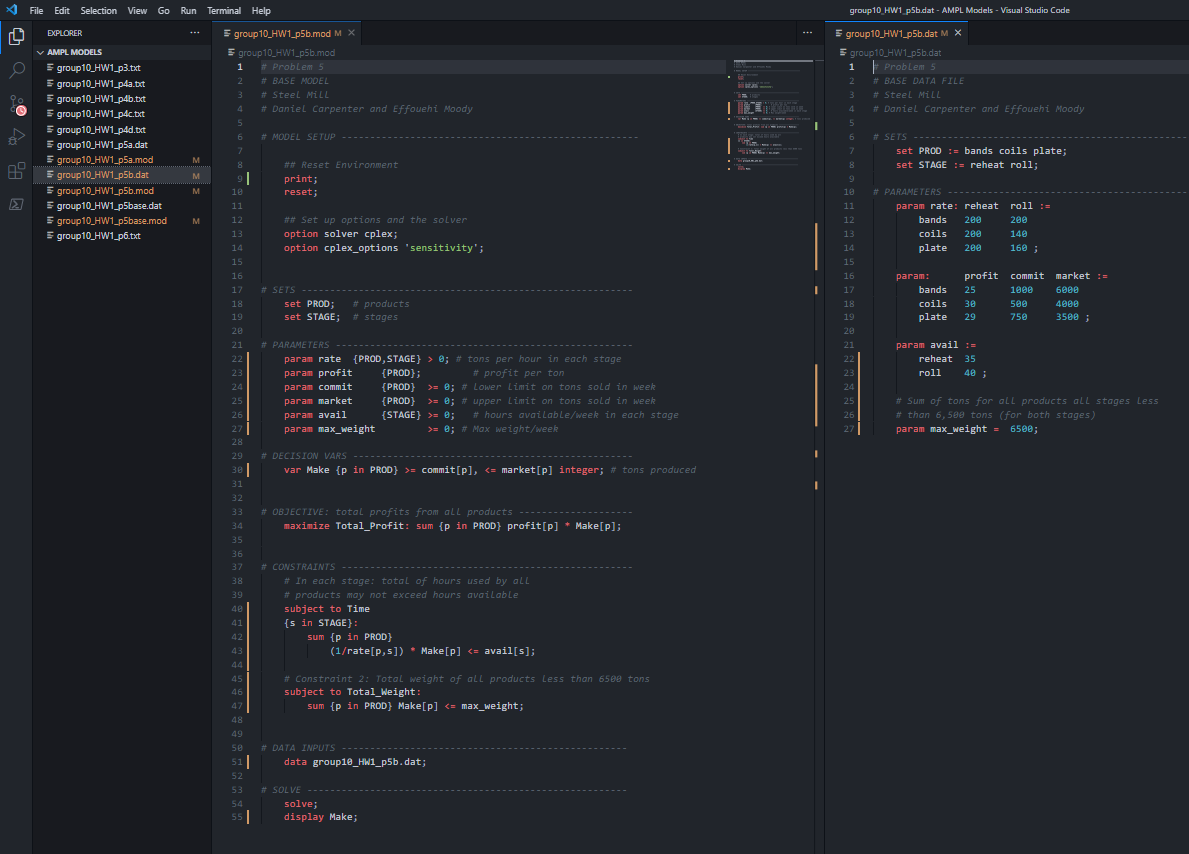
\includegraphics{"Output_Images/codeProblem5b.png}
\caption{Image}
\end{figure}

\hypertarget{output-6}{%
\subsubsection{Output}\label{output-6}}

\begin{quote}
The total number of tons has reduced from 7,000 to 6,500 per week
\end{quote}

\begin{figure}
\centering
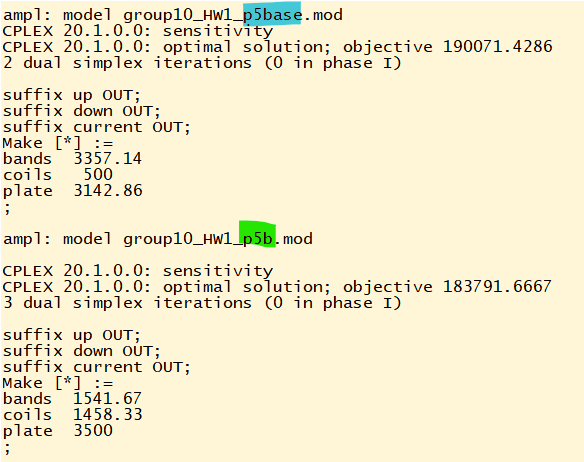
\includegraphics{"Output_Images/outputProblem5b.png}
\caption{Image}
\end{figure}

\hypertarget{task-c-1}{%
\subsection{\texorpdfstring{Task \texttt{c}}{Task c}}\label{task-c-1}}

\hypertarget{changed-objective-function}{%
\subsubsection{Changed Objective
Function}\label{changed-objective-function}}

\begin{itemize}
\tightlist
\item
  \emph{Change the objective function to maximize total tons}
\end{itemize}

\[
maximize \ Total\_Tons = \sum_{p \ \in \ PROD} Make_{p}
\]

\hypertarget{code-7}{%
\subsubsection{Code}\label{code-7}}

\begin{figure}
\centering
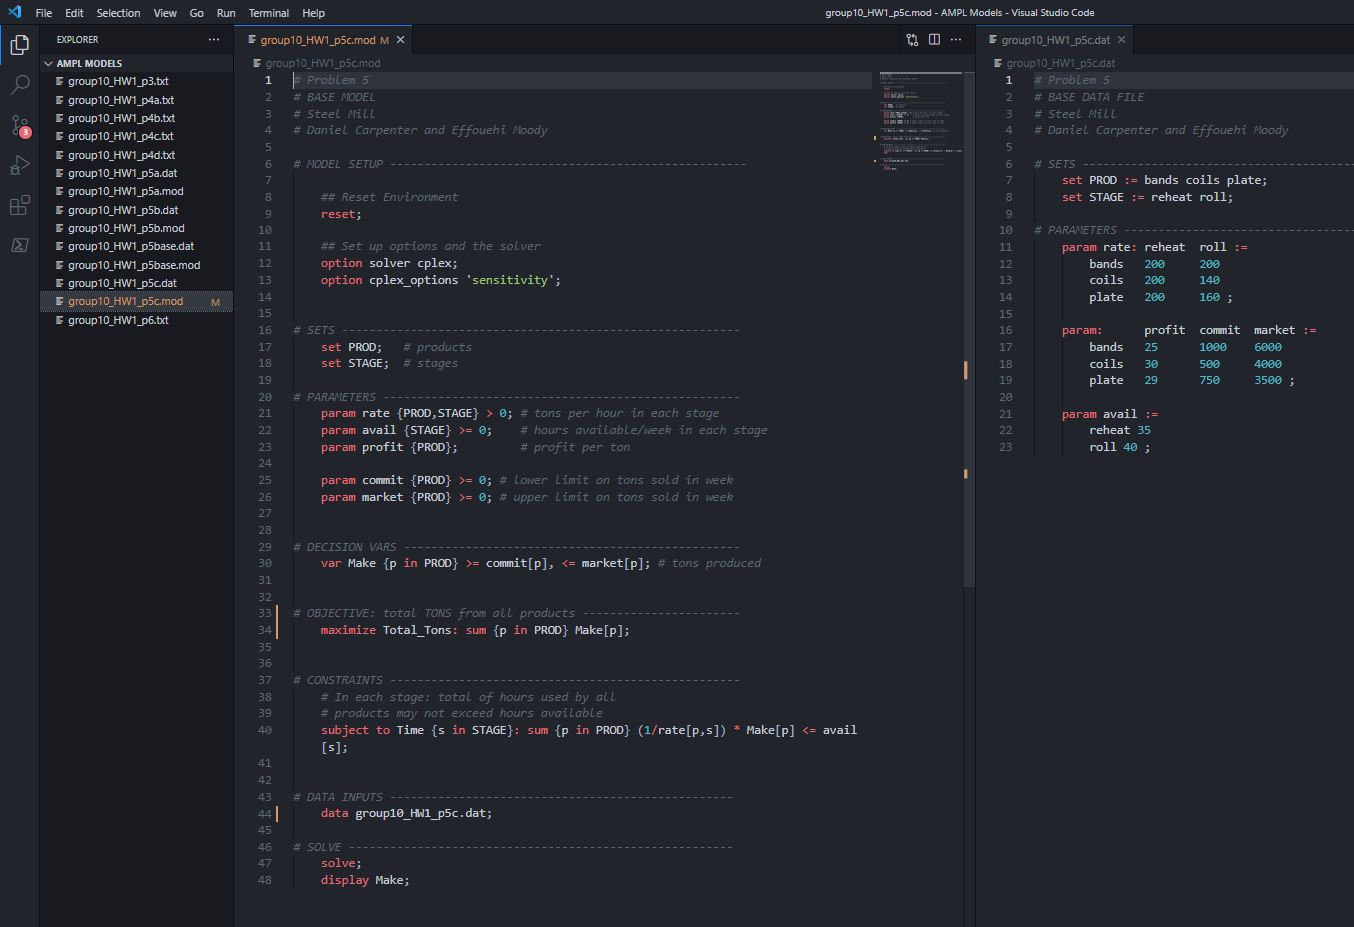
\includegraphics{"Output_Images/codeProblem5c.png}
\caption{Image}
\end{figure}

\hypertarget{output-7}{%
\subsubsection{Output}\label{output-7}}

\begin{quote}
The data file does not make a diference in the optimal (assuming that is
what the question is asking). Please note that the total number of tons
produced are the same as in the \texttt{base} model; however, the
allocation of tons have shifted among each of the products.
\end{quote}

\begin{figure}
\centering
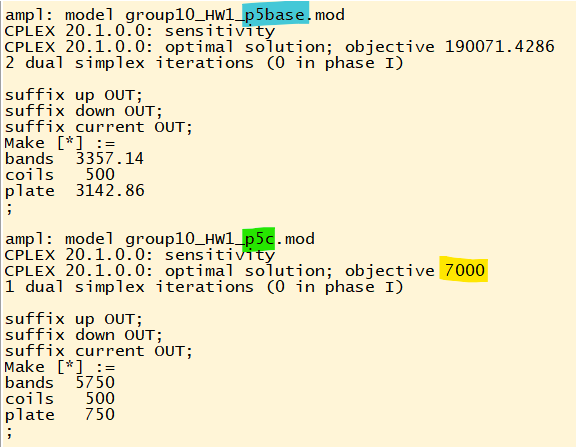
\includegraphics{"Output_Images/outputProblem5c.png}
\caption{Image}
\end{figure}

\hypertarget{task-d-1}{%
\subsection{\texorpdfstring{Task \texttt{d}}{Task d}}\label{task-d-1}}

\hypertarget{new-constraint}{%
\subsubsection{New Constraint}\label{new-constraint}}

\begin{itemize}
\tightlist
\item
  \emph{Minimum Share of Tons for each Product}
\end{itemize}

\[
Share\_of\_Products: Make_{j} \geq share_{j} \times 
\sum_{k \ \in \ PROD} Make_{k}, \ \  \forall \ j \ \in \ PROD
\]

\hypertarget{code-part-i}{%
\subsubsection{Code (Part I)}\label{code-part-i}}

\begin{figure}
\centering
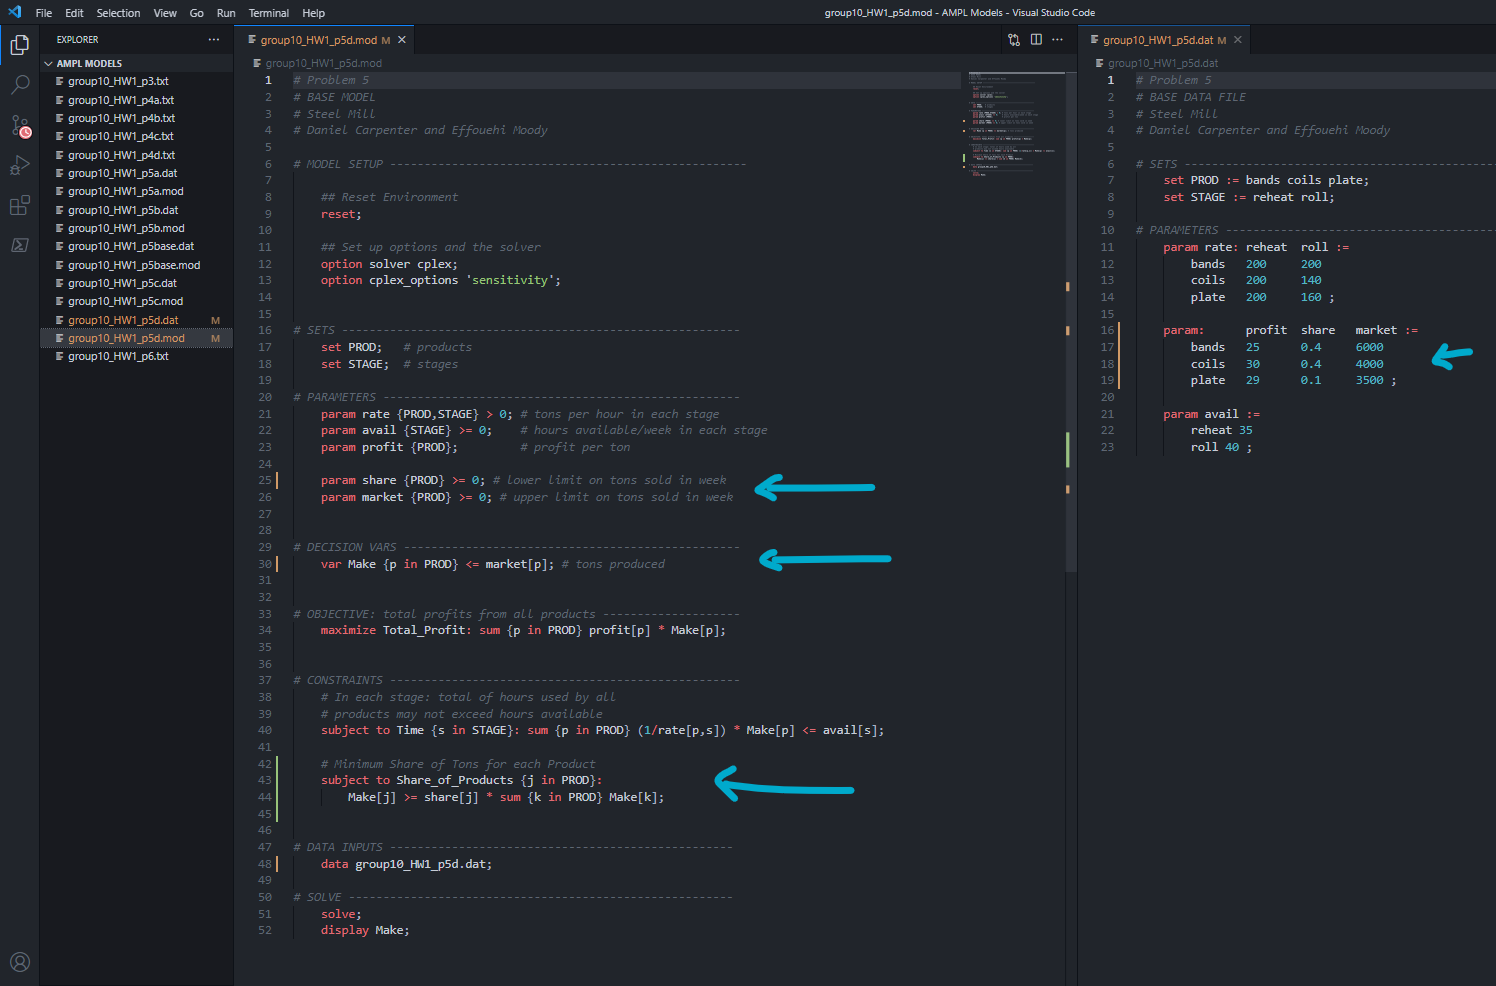
\includegraphics{"Output_Images/codeProblem5d.png}
\caption{Image}
\end{figure}

\hypertarget{output-part-i}{%
\subsubsection{Output (Part I)}\label{output-part-i}}

\begin{quote}
Note that bands represent \textasciitilde49.99\%, coils: 40\%, and
plates: 10\%
\end{quote}

\begin{figure}
\centering
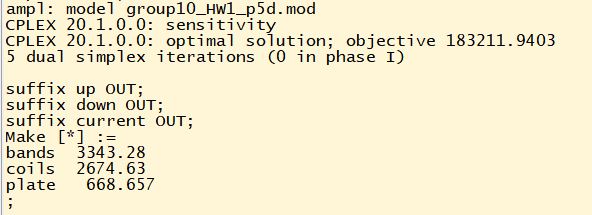
\includegraphics{"Output_Images/outputProblem5d.png}
\caption{Image}
\end{figure}

\hypertarget{code-part-ii}{%
\subsubsection{Code (Part II)}\label{code-part-ii}}

\begin{figure}
\centering
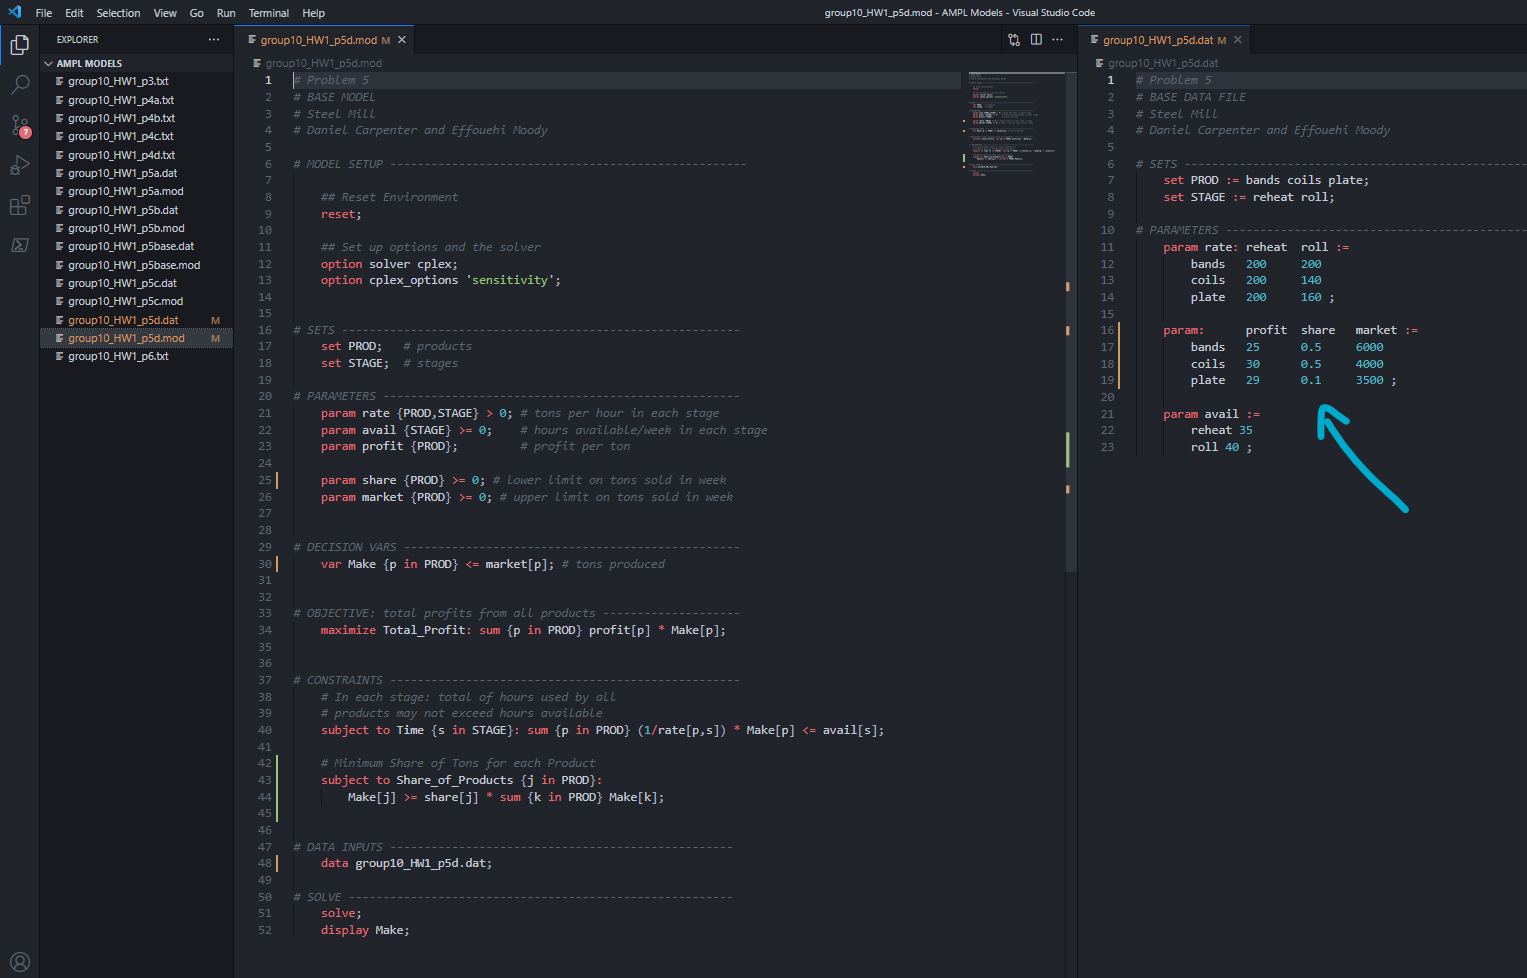
\includegraphics{"Output_Images/codeProblem5d1.png}
\caption{Image}
\end{figure}

\hypertarget{output-part-ii}{%
\subsubsection{Output (Part II)}\label{output-part-ii}}

\begin{quote}
Profit is zero because it is impossible for bands to reach 50\% of the
share.
\end{quote}

\begin{figure}
\centering
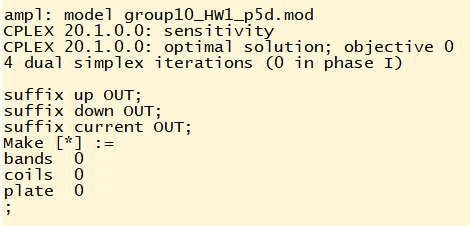
\includegraphics{"Output_Images/outputProblem5d1.png}
\caption{Image}
\end{figure}

\hypertarget{task-e}{%
\subsection{\texorpdfstring{Task \texttt{e}}{Task e}}\label{task-e}}

\hypertarget{changing-input-data-via-.dat-file}{%
\subsubsection{\texorpdfstring{Changing Input Data via \texttt{.dat}
File}{Changing Input Data via .dat File}}\label{changing-input-data-via-.dat-file}}

\begin{quote}
Simply add the new item within the set called \texttt{finishing}, then
add the its the associate values to the \texttt{rate} and \texttt{avail}
parameters.
\end{quote}

\begin{figure}
\centering
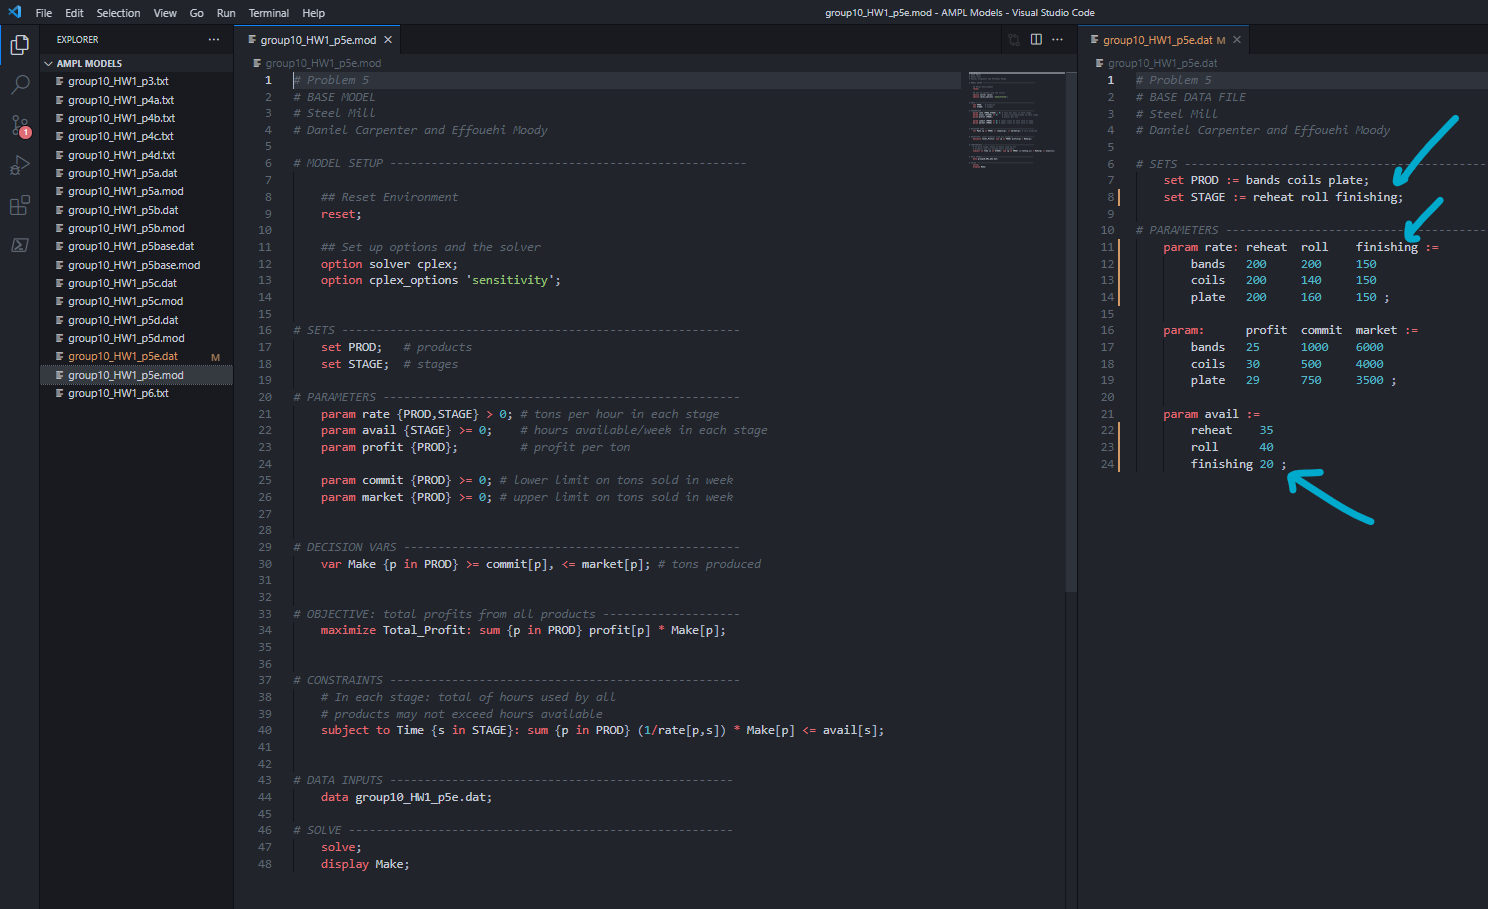
\includegraphics{"Output_Images/codeProblem5e.png}
\caption{Image}
\end{figure}

\hypertarget{output-8}{%
\subsubsection{Output}\label{output-8}}

\begin{figure}
\centering
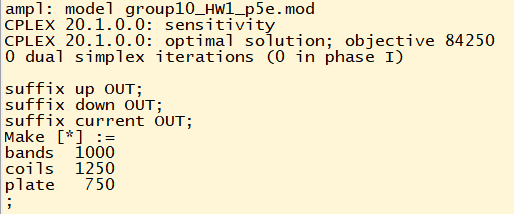
\includegraphics{"Output_Images/outputProblem5e.png}
\caption{Image}
\end{figure}

\begin{center}\rule{0.5\linewidth}{0.5pt}\end{center}

\hypertarget{problem-6}{%
\section{\texorpdfstring{Problem
\texttt{6}}{Problem 6}}\label{problem-6}}

\begin{center}\rule{0.5\linewidth}{0.5pt}\end{center}

\hypertarget{task-a---c}{%
\subsection{\texorpdfstring{Task \texttt{a} -
\texttt{c}}{Task a - c}}\label{task-a---c}}

\hypertarget{decision-variables-3}{%
\subsubsection{Decision Variables}\label{decision-variables-3}}

\texttt{bondA}: dollars \(\in \mathbb{R}\) to invest in bond A\\
\texttt{bondB}: dollars \(\in \mathbb{R}\) to invest in bond B\\
\texttt{bondC}: dollars \(\in \mathbb{R}\) to invest in bond C\\
\texttt{bondD}: dollars \(\in \mathbb{R}\) to invest in bond D\\
\texttt{bondE}: dollars \(\in \mathbb{R}\) to invest in bond E

\hypertarget{objective-function-3}{%
\subsubsection{Objective Function}\label{objective-function-3}}

\begin{itemize}
\tightlist
\item
  Maximize the Expected Earnings of the portfolio
\end{itemize}

\[
Maximize \ Z = (0.043 \times bondA) + (0.027 \times bondB) + (0.025 \times bondC) + (0.022 \times bondD) + (0.045 \times bondE)
\]

\hypertarget{constraints-2}{%
\subsubsection{Constraints}\label{constraints-2}}

\textbf{C1:} Budget to invest is \$10 MM or less \[
budget: bondA + bondB + bondC + bondD + bondE \leq 10
\]

\textbf{C2:} At least \$4 million must be invested in government and
agency bonds \[
govtAndAgency: bondB + bondC + bondD \geq 4
\]

\textbf{C3:} Average Quality of the Portfolio must not exceed 1.4 \[
avgQuality: (0.6 \times bondA) + (0.6 \times bondB) - (0.4 \times bondC) 
- (0.4 \times bondD) + (3.6 \times bondE) \leq 0
\]

\textbf{C4:} The Average Maturity must not Exceed Five Years \[
avgMaturity: (4 \times bondA) + (10 \times bondB) - (1 \times bondC) 
- (2 \times bondD) - (3 \times bondE) \leq 0
\]

\textbf{C5:} Only select Bonds A and D (Don't select B, C, or E) \[
onlyAandB: bondB + bondC + bondE = 0;
\]

\textbf{C6:} Municipal Bonds must be less than or equal to \$3 MM \[
municipal: bondA \leq 3;
\]

\hypertarget{code-8}{%
\subsubsection{Code}\label{code-8}}

\begin{figure}
\centering
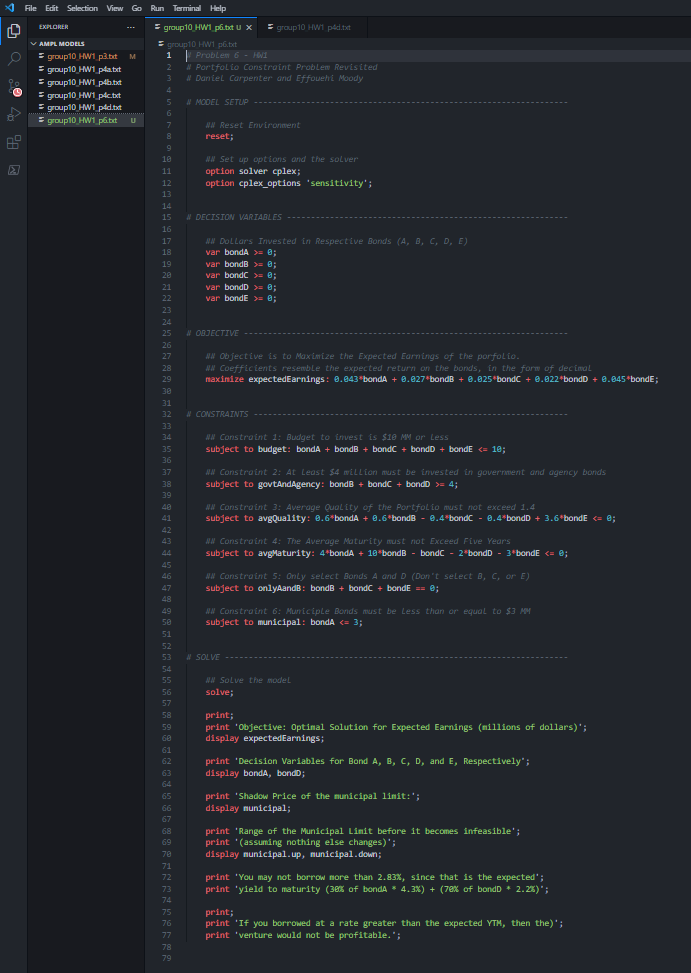
\includegraphics{"Output_Images/codeProblem6.png}
\caption{Image}
\end{figure}

\hypertarget{output-9}{%
\subsubsection{Output}\label{output-9}}

\begin{figure}
\centering
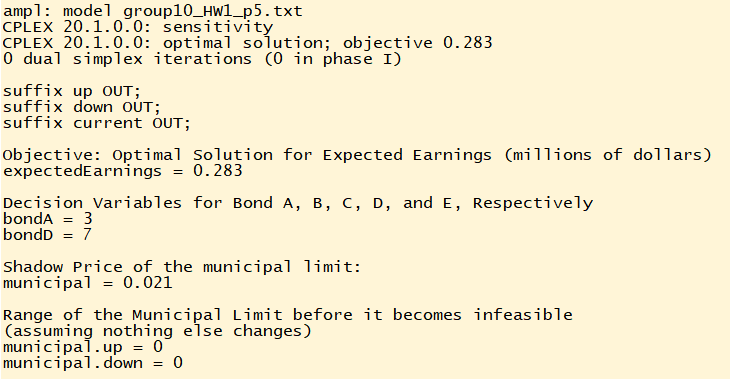
\includegraphics{"Output_Images/outputProblem6.png}
\caption{Image}
\end{figure}

\hypertarget{task-d-2}{%
\subsection{\texorpdfstring{Task \texttt{d}:}{Task d:}}\label{task-d-2}}

You may not borrow more than 2.83\%, since that is the expected\\
yield to maturity (30\% of bondA * 4.3\%) + (70\% of bondD * 2.2\%)

\hypertarget{task-e-1}{%
\subsection{\texorpdfstring{Task \texttt{e}:}{Task e:}}\label{task-e-1}}

If you borrowed at a rate greater than the expected YTM, then the\\
venture would not be profitable.

\end{document}
